\scanpage{52}\mspage{11}
(A5) l'orientation $\omega_{J,i}$ de $K_{\unsure{Ji|J}}$ est indépendante
du choix de $i$.
% slanted
\margin{Si on désigne par $\alpha,\beta,\gamma$ les intersections de $D_i$ avec les trois ps-droites de $K_J$, et par $\unsure{\lambda_\alpha|\lambda\alpha|\partial\alpha},\lambda_\beta,\lambda_\gamma$ les arêtes de $K_I$ qui les contiennent $\{\lambda_\alpha,\lambda_\beta,\lambda_\gamma\}$ c'est \unsure{par|là} l'orientation}

\uline{2\textsuperscript{ième} cas} Toute ps. droite de $K$ passe par
un des trois sommets de $K_J$.
Comme on suppose qu'il n'y a
pas de bigône dans $K$, on
trouve d'ailleurs que par chaque
sommet, il passe au moins une
$D_i$ avec $i\in I\setminus J$.
\figure{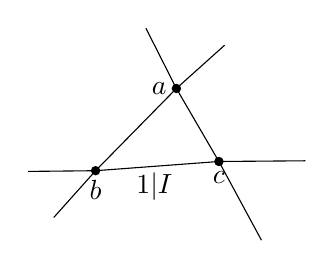
\begin{tikzpicture}[x=.009cm,y=-.009cm]
\draw (8,244)--(103,243)--(277,230)--(399,229); \draw (44,309)--(103,243)--(217,127)--(285,66); \draw (174,42)--(217,127)--(277,230)--(337,341);
\fill (217,127) circle (1.7pt) node[left] {$a$}; \fill (103,243) circle (1.7pt) node[below] {$b$};
\fill (277,230) circle (1.7pt) node[below] {$c$}; \node at (186,266) {$\unsure{1|I}$};
\end{tikzpicture}}

Supposons d'abord qu'on peut trouver
des droites $D_a,D_b,D_c$ passant par les
sommets $a,b,c$, qui ne soient pas concourantes.
On trouve une configuration,
associée canoniquement à l'ens
$J$ à trois éléments, avec comme
\inserted{9} sommets les $a_i$ $(i\in J)$ de
$K_J$, les intersections $\alpha_i$ $(i\in J)$
des $D_{a_i}$ avec $D_i$ (\uline{NB} $a_i$ est
le sommet de $K_J$ opposé à $D_i$)
\figure{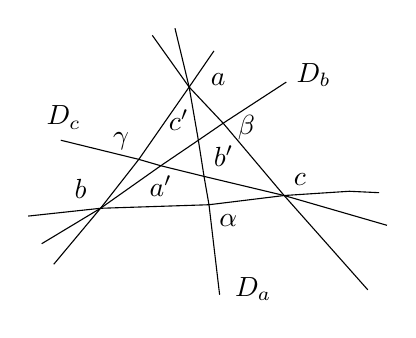
\begin{tikzpicture}[x=.009cm,y=-.009cm]
\draw (70,373)--(136,294)--(190,225)--(261,123)--(296,72);
\draw (209,50)--(261,123)--(309,174)--(395,276)--(513,409);
\draw (34,305)--(136,294)--(289,289)--(395,276)--(487,270)--(529,272);
\draw (241,40)--(261,123)--(274,198)--(282,249)--(289,289)--(304,416);
\draw (53,344)--(136,294)--(221,234)--(274,198)--(309,174)--(398,116);
\draw (80,198)--(190,225)--(221,234)--(282,249)--(395,276)--(540,318);
\node[right] at (278,113) {$a$}; \node[above left] at (130,294) {$b$};
\node[above right] at (395,276) {$c$}; \node[right] at (399,106) {$D_b$};
\node[above] at (84,196) {$D_c$}; \node[right] at (312,408) {$D_a$};
\node[below right] at (290,289) {$\alpha$}; \node[right] at (316,180) {$\beta$};
\node[above left] at (190,225) {$\gamma$}; \node[below] at (221,234) {$a'$};
\node[above right] at (282,249) {$b'$}; \node[above left] at (274,198) {$c'$};
\end{tikzpicture}}
les $a'_i$ $(i\in J)$ intersections de $D^{\unsure{\prime|1}}_{a_j}$ et $D_{a_{\deleted{\unsure{j}}k}}$ (où
$J=\{i,j,\unsure{h|k}\}$). \deleted{\unsure{L}} La figure montre comment
les sommets se répartissent suivant les 6
ps. droites $D_i,D_{a_i}$, et \deleted{la configuration est} \inserted{le $D_{J'}$ correspondant}
(avec les 6 ps. droites) est compl\textsuperscript{t} décrit,
quand on a décrit les structures polygônales
% archive sheet number: 51
